\documentclass[aspectratio=169]{../latex_main/tntbeamer}  % you can pass all options of the beamer class, e.g., 'handout' or 'aspectratio=43'
\usepackage{dsfont}
\usepackage{bm}
\usepackage[english]{babel}
\usepackage[T1]{fontenc}
%\usepackage[utf8]{inputenc}
\usepackage{graphicx}
\graphicspath{ {./figures/} }
\usepackage{algorithm}
\usepackage[ruled,vlined,algo2e,linesnumbered]{algorithm2e}
\usepackage{hyperref}
\usepackage{booktabs}
\usepackage{mathtools}

\usepackage{amsmath,amssymb}

\DeclareMathOperator*{\argmax}{arg\,max}
\DeclareMathOperator*{\argmin}{arg\,min}

\usepackage{amsbsy}
\newcommand{\vect}[1]{\bm{#1}}
%\newcommand{\vect}[1]{\boldsymbol{#1}}

\usepackage{pgfplots}
\pgfplotsset{compat=1.16}
\usepackage{tikz}
\usetikzlibrary{trees} 
\usetikzlibrary{shapes.geometric}
\usetikzlibrary{positioning,shapes,shadows,arrows,calc,mindmap}
\usetikzlibrary{positioning,fadings,through}
\usetikzlibrary{decorations.pathreplacing}
\usetikzlibrary{intersections}
\pgfdeclarelayer{background}
\pgfdeclarelayer{foreground}
\pgfsetlayers{background,main,foreground}
\tikzstyle{activity}=[rectangle, draw=black, rounded corners, text centered, text width=8em]
\tikzstyle{data}=[rectangle, draw=black, text centered, text width=8em]
\tikzstyle{myarrow}=[->, thick, draw=black]

% Define the layers to draw the diagram
\pgfdeclarelayer{background}
\pgfdeclarelayer{foreground}
\pgfsetlayers{background,main,foreground}

% Requires XeLaTeX or LuaLaTeX
%\usepackage{unicode-math}

\usepackage{fontspec}
%\setsansfont{Arial}
\setsansfont{RotisSansSerifStd}[ 
Path=../latex_main/fonts/,
Extension = .otf,
UprightFont = *-Regular,  % or *-Light
BoldFont = *-ExtraBold,  % or *-Bold
ItalicFont = *-Italic
]
\setmonofont{Cascadia Mono}[
Scale=0.8
]

% scale factor adapted; mathrm font added (Benjamin Spitschan @TNT, 2021-06-01)
%\setmathfont[Scale=1.05]{Libertinus Math}
%\setmathrm[Scale=1.05]{Libertinus Math}

% other available math fonts are (not exhaustive)
% Latin Modern Math
% XITS Math
% Libertinus Math
% Asana Math
% Fira Math
% TeX Gyre Pagella Math
% TeX Gyre Bonum Math
% TeX Gyre Schola Math
% TeX Gyre Termes Math

% Literature References
\newcommand{\lit}[2]{\href{#2}{\footnotesize\color{black!60}[#1]}}

%%% Beamer Customization
%----------------------------------------------------------------------
% (Don't) Show sections in frame header. Options: 'sections', 'sections light', empty
\setbeamertemplate{headline}{empty}

% Add header logo for normal frames
\setheaderimage{
	% 
\includegraphics[height=\logoheight]{figures/TNT_darkv4.pdf}
	
\includegraphics[height=\logoheight]{../latex_main/figures/luh_logo_rgb_0_80_155.pdf}
	% 
\includegraphics[height=\logoheight]{figures/logo_tntluh.pdf}
}

% Header logo for title page
\settitleheaderimage{
	% 
\includegraphics[height=\logoheight]{figures/TNT_darkv4.pdf}
	
\includegraphics[height=\logoheight]{../latex_main/figures/luh_logo_rgb_0_80_155.pdf}
	% 
\includegraphics[height=\logoheight]{figures/logo_tntluh.pdf}
}

% Title page: tntdefault 
\setbeamertemplate{title page}[tntdefault]  % or luhstyle
% Add optional title image here
%\addtitlepageimagedefault{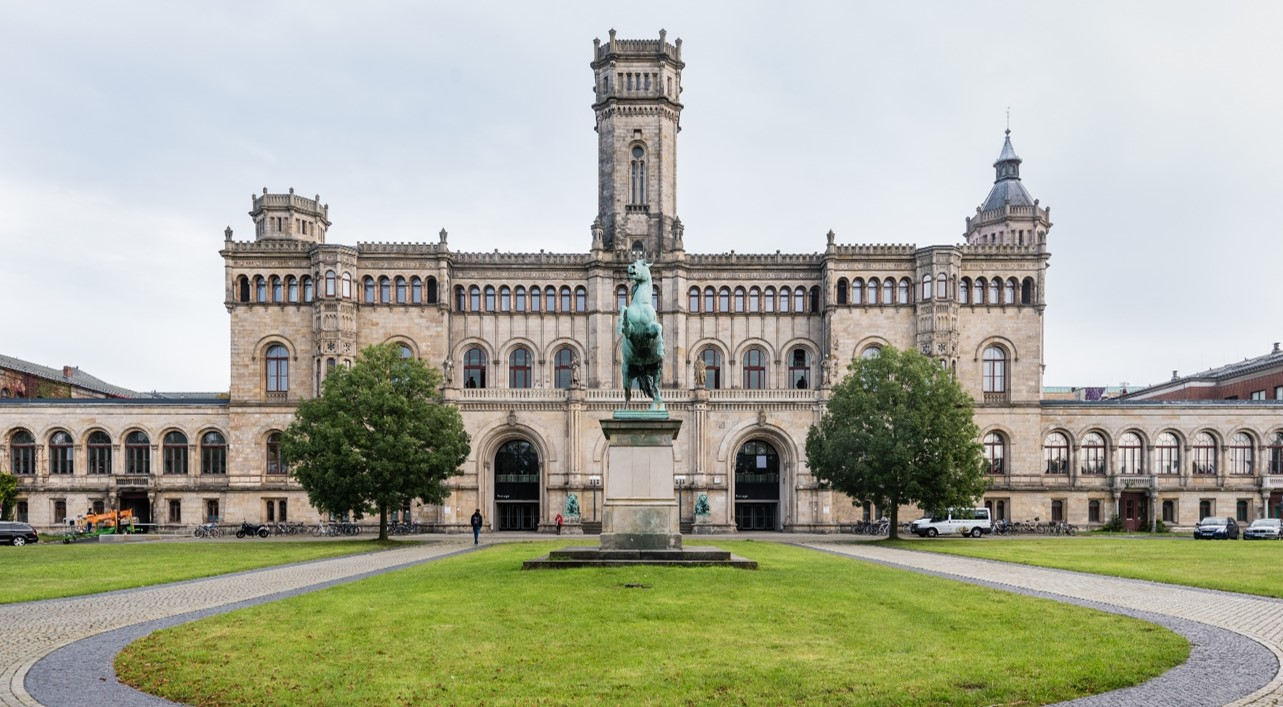
\includegraphics[width=0.65\textwidth]{figures/luh_default_presentation_title_image.jpg}}

% Title page: luhstyle
% \setbeamertemplate{title page}[luhstyle]
% % Add optional title image here
% \addtitlepageimage{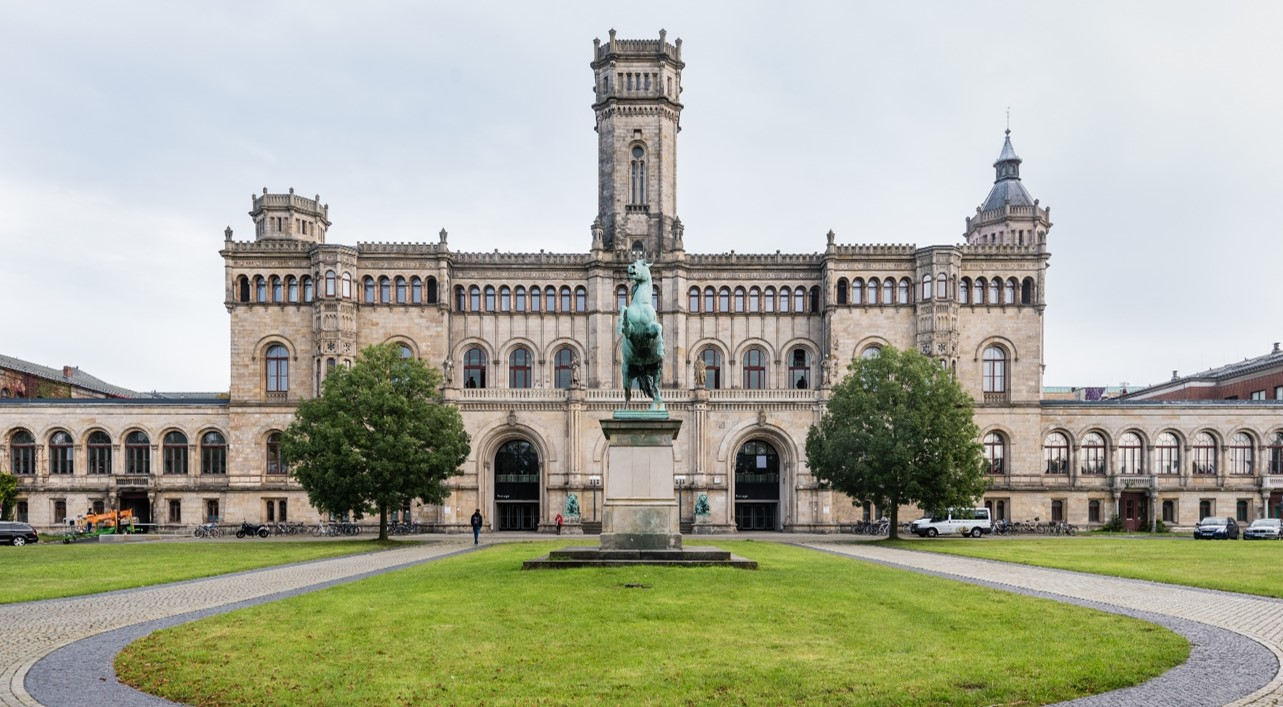
\includegraphics[width=0.75\textwidth]{figures/luh_default_presentation_title_image.jpg}}

\author[Abedjan \& Lindauer]{Ziawasch Abedjan \& Marius Lindauer\\[1em]
	
\includegraphics[height=\logoheight]{../latex_main/figures/luh_logo_rgb_0_80_155.pdf}\qquad
	
\includegraphics[height=\logoheight]{../latex_main/figures/DBIS_Kurzlogo.png}\qquad

\includegraphics[height=\logoheight]{../latex_main/figures/TNT_darkv4}\qquad

\includegraphics[height=\logoheight]{../latex_main/figures/L3S.jpg}	}
\date{Summer Term 2022; \hspace{0.5em} {
\includegraphics[height=1.5em]{../latex_main/figures/Cc-by-nc-sa_icon.svg.png}}; based on \href{https://ds100.org/fa21/}{[DS100]}
}


%%% Custom Packages
%----------------------------------------------------------------------
% Create dummy content
\usepackage{blindtext}

% Adds a frame with the current page layout. Just call \layout inside of a frame.
\usepackage{layout}


%%% Macros
%\renewcommand{\vec}[1]{\mathbf{#1}}
% \usepackage{bm}
%\let\vecb\bm

\title[Regression]{DS: Ordinary Least Squares}
\subtitle{Geometric derivation (Optional)}

\graphicspath{ {./figure_ols/} }
%\institute{}


\begin{document}
	
	\maketitle
	\begin{frame}{A linear combination of columns}
	    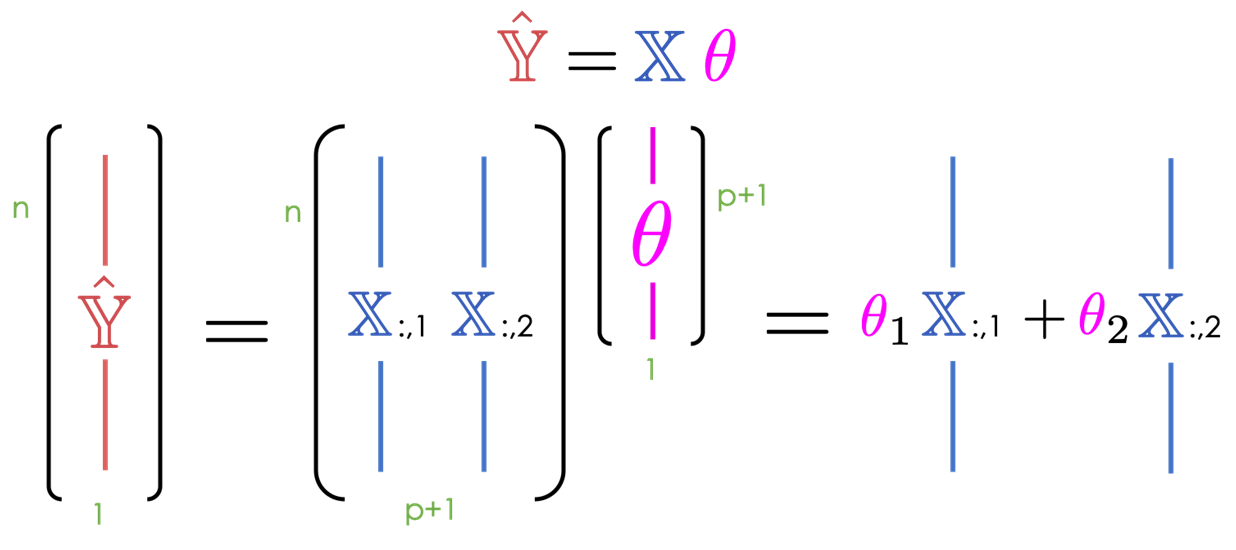
\includegraphics[scale=.4]{Bild5}\\
	    The linear model represents  ${\hat{\vect{Y}}}$     as a linear combination of the columns of     $\vect{X}$ 
	\end{frame}
	
	\begin{frame}{Span}
	    \begin{columns}
	        \begin{column}{.5\textwidth}
	                Our prediction is a linear combination of the columns of $\vect{X}$. 
	                \begin{itemize}
	                    \item The set of all possible linear combinations of the columns of $\vect{X}$ is called the span of the columns of $\vect{X}$ (denoted      $span(\vect{X})$           ).
	                    \begin{itemize}
	                        \item Also called the column space
	                    \end{itemize}
                        \item Intuitively, this is all of the vectors you can “reach” using the columns of $\vect{X}$.
                        \item Since each column of $\vect{X}$ has length $n$, $span(\vect{X})$ is a subspace of $\mathbb{R}^n$    
                        \item Our goal is to find the vector in $span(\vect{X})$ that is closest to  $\vect{Y}$. 
	                \end{itemize}
	        \end{column}
	        \begin{column}{.4\textwidth}
	                \begin{figure}
	                    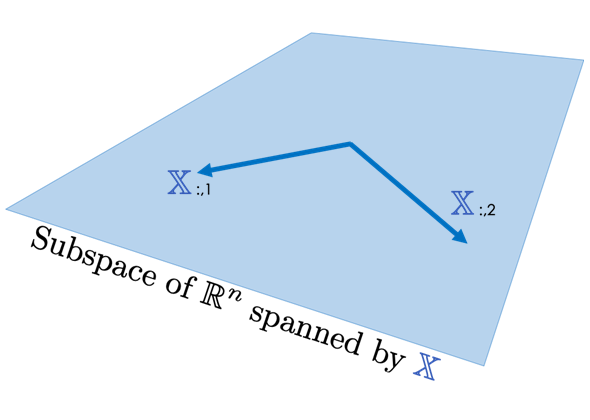
\includegraphics[scale=.45]{Bild6}
	                \end{figure}
	        \end{column}
	    \end{columns}
	\end{frame}
	 
	 
	 \begin{frame}{Geometry View}
	    \begin{columns}
	        \begin{column}{.6\textwidth}
	               \begin{figure}
	                    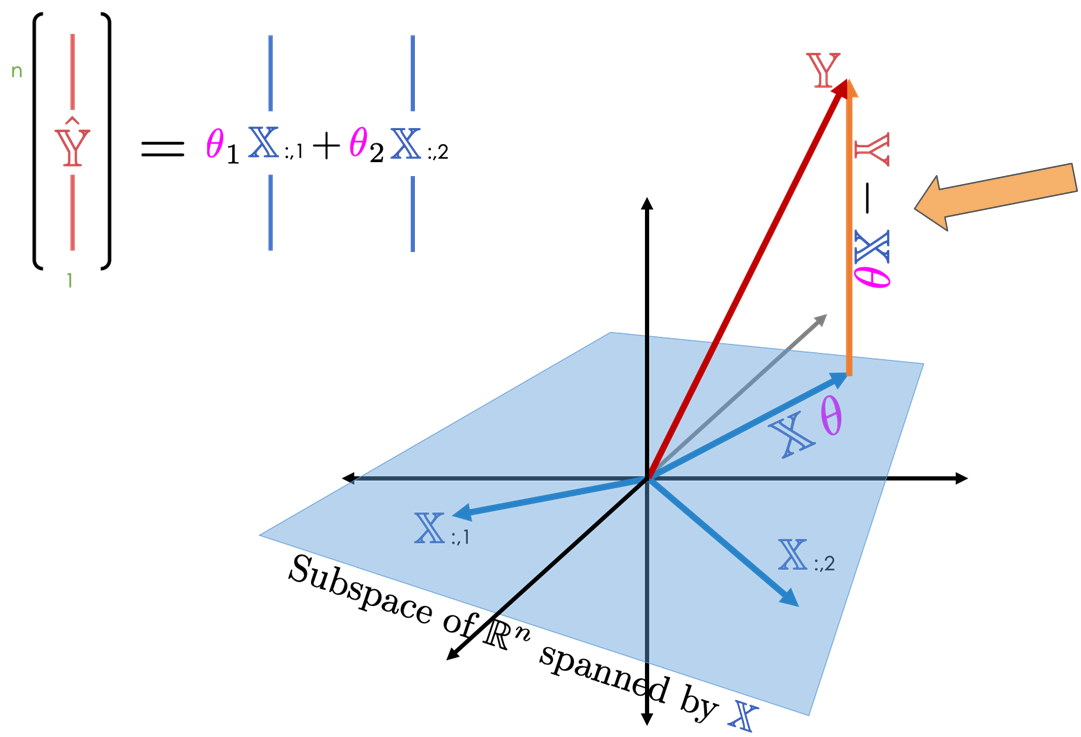
\includegraphics[scale=.3]{Bild7}
	                \end{figure}
	        \end{column}
	        \begin{column}{.3\textwidth}
	                Recall, this is the residual vector,
                    \begin{equation*}
                        e = \vect{Y} - {\hat{\vect{Y}}}
                    \end{equation*}
                    Our goal is to minimize the $L_2$ norm of the residual vector, i.e. we want our predictions to be “as close” to our true y values as possible.

	        \end{column}
	    \end{columns}
	\end{frame}
	
	
	 \begin{frame}{Geometry View}
	    \centering
	    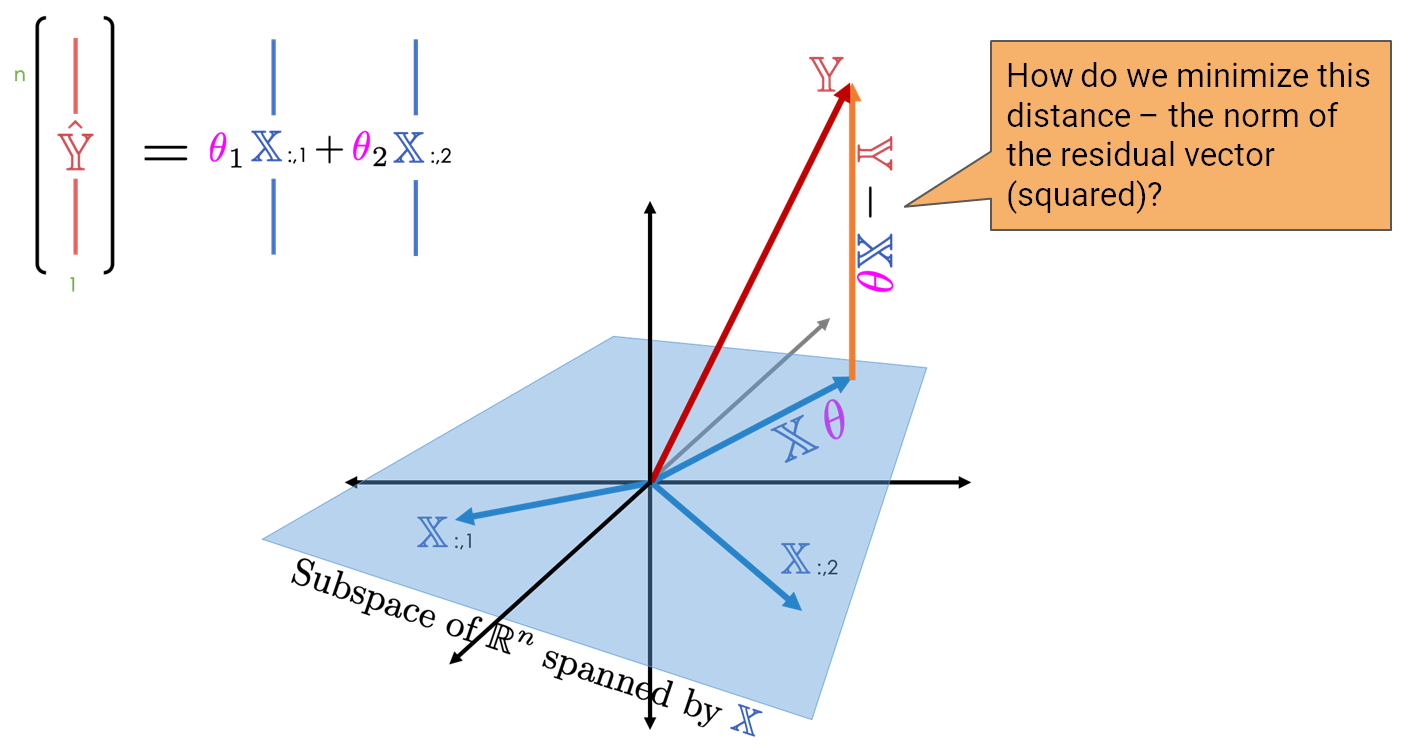
\includegraphics[scale=.33]{Bild8}
	\end{frame}
	
	
	\begin{frame}{Geometry View}
	    \centering
	    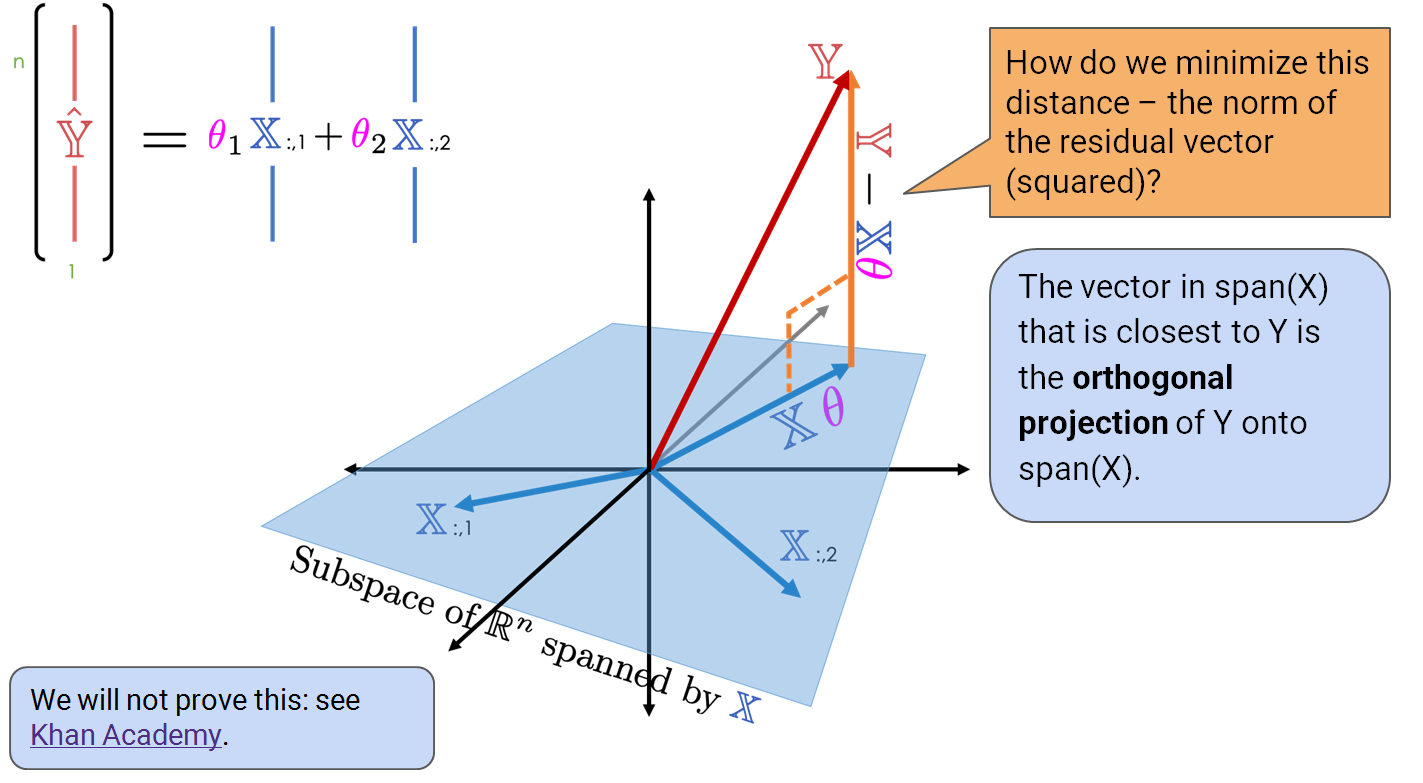
\includegraphics[scale=.32]{Bild9}
	\end{frame}
	
	\begin{frame}{Geometry View}
	    \centering
	    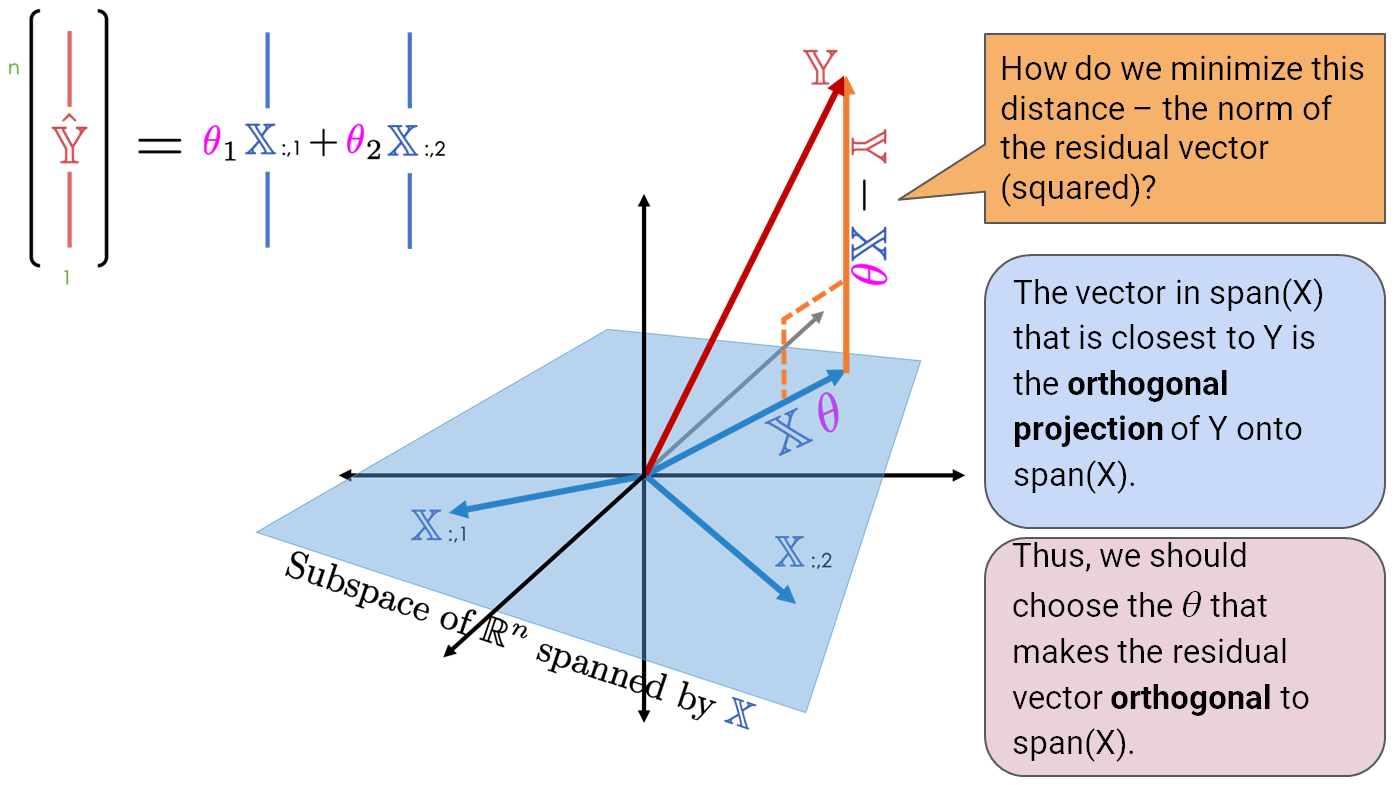
\includegraphics[scale=.32]{Bild10}
	\end{frame}
	
	
	
	\begin{frame}{Orthogonality}
	    We say two vectors are orthogonal if and only if their dot product is 0.
	    \begin{itemize}
	        \item This is a generalization of the notion of two vectors in 2D being perpendicular.
	    \end{itemize}
	    \begin{equation*}
	        \vect{a}^\intercal\vect{b} = 0 \Leftrightarrow \vect{a},\vect{b} \text{ are orthogonal}
	    \end{equation*}
	    Suppose a vector is orthogonal to the span of the columns of a matrix.
	    \begin{itemize}
	        \item This is true if and only if it is orthogonal to each column individually. 
	        \item Let $\vect{M} \in \mathbb{R}^{n\times d}, \vect{v} \in \mathbb{R}^{n\times 1}$. Suppose $v$ is orthogonal to the span of the columns of $\vect{M}$. Then:
	    \end{itemize}
	    \begin{align*}
    	   \vect{M} =  \left[\begin{array}{cccc}
                \vdots & \vdots & \vdots & \vdots\\
                \vect{m}_1 &  \vect{m}_2 & \dots & \vect{m}_d\\
                \vdots & \vdots & \vdots & \vdots
            \end{array}\right]
            \begin{array}{c}
                \vect{m}_1^\intercal \vect{v} = 0\\
                \vect{m}_2^\intercal \vect{v} = 0\\
                \vdots\\
                \vect{m}_d^\intercal \vect{v} = 0\\
            \end{array}
            \rightarrow \vect{M}^\intercal \vect{v} = \Vec{0}
         \end{align*}
	\end{frame}
	
	
	\begin{frame}{Orthogonality}
	\vspace{-2em}
	Let $\vect{M} \in \mathbb{R}^{n\times d}, \vect{v} \in \mathbb{R}^{n\times 1}$.  Suppose $\vect{v}$ is orthogonal to the span of the columns of $\vect{M}$.
	    \begin{align*}
	   \vect{M} =  \left[\begin{array}{cccc}
                \vdots & \vdots & \vdots & \vdots\\
                \vect{m}_1 &  \vect{m}_2 & \dots & \vect{m}_d\\
                \vdots & \vdots & \vdots & \vdots
            \end{array}\right]
            \end{align*}
            
            $v$ is orthogonal to each column of $M$ separately. 
(Note, each column of $M$ has length $n$, and $\vect{v}$ also has length $n$).
        \begin{equation*}
            \begin{array}{c}
                \vect{m}_1^\intercal \vec{v} = 0\\
                \vect{m}_2^\intercal \vect{v} = 0\\
                \vdots\\
                \vect{m}_d^\intercal \vect{v} = 0\\
            \end{array}
        \end{equation*}
            This product encapsulates all d of the equations on the left into a single equation. The quantity on the right is the zero vector (d-length vector full of 0s).
            \begin{align*}
                 \vect{M}^\intercal \vect{v} = \Vec{0}
            \end{align*}
	\end{frame}
	
	
	\begin{frame}{Residuals are orthogonal to the span of X}
	We want the $\vect{\theta}$ such that the residual vector is orthogonal to  span($\vect{X}$)\\
	\bigskip
	By the definition of orthogonality:
    $\vect{X}^\intercal(\vect{Y} - \vect{X}\hat{\vect{\theta}}) = \Vec{0}$\\
    \bigskip
    Rearranging: $\vect{X}^\intercal\vect{Y} - \vect{X}^\intercal\vect{X}\hat{\vect{\theta}} = \Vec{0}$\\
    \bigskip
    The normal equation: $\vect{X}^\intercal\vect{X}\hat{\vect{\theta}} = \vect{X}^\intercal\vect{Y} $\\
    \bigskip
    Assuming     $\vect{X}^\intercal\vect{X}$       is full rank: $\hat{\vect{\theta}} = (\vect{X}^\intercal\vect{X})^{-1} \vect{X}^\intercal\vect{Y} $\\

	\end{frame}
	
	\begin{frame}[c]{OLS Estimate}
	\begin{equation*}
	   \hat{\theta} = (\vect{X}^\intercal\vect{X})^{-1} \vect{X}^\intercal\vect{Y} 
	\end{equation*}
	This result is so important, it deserves its own slide.
It is the least squares estimate for $\vect{\theta}$.

    \bigskip
    \alert{Warning}: You have to compute $(\vect{X}^\intercal\vect{X})^{-1}$, which takes $\mathcal{O}(n^3)$ $\leadsto$ not feasible for many features!

	\end{frame}
	
	
	\begin{frame}{Summary}
	    1. Choose a model. We chose the multiple linear regression model, formulated using a matrix.
        \begin{equation*}
            \hat{\vect{Y}} = \vect{X}\vect{\theta}
        \end{equation*}
        2. Choose a loss function. We chose squared loss, and hence our average loss was
        \begin{equation*}
            R(\theta) = \frac{1}{n}||\vect{Y} - \vect{\hat{Y}}||_2^2 = \frac{1}{n}||\vect{Y} - \vect{X}\vect{\theta}||_2^2
        \end{equation*}
        
        3. Minimize average loss to determine optimal model parameters. Done!
        \begin{equation*}
	        \hat{\vect{\theta}} = (\vect{X}^\intercal\vect{X})^{-1} \vect{X}^\intercal\vect{Y} 
	    \end{equation*}
	\end{frame}
\end{document}